% Define the module top matter
% This gets used to create the chapter title page
% NOTES:
%  * When multiple people have authored or contributed to the module, simply use a LaTeX line break
%    (a double-backslash: \\) at the end of each person.
%  * If you don't want this information shown on the module chapter page, simply remove the lines
%    within the \setModuleAuthors{} and \setModuleContributions{} environments
\setModuleTitle{Introduction to Nextflow}
\setModuleAuthors{%
  Rados{\l}aw Suchecki \mailto{rad.suchecki@csiro.au}
}
\setModuleContributions{%
%  John Doe \mailto{john.dow@example.com}%
}

% BEGIN: Module Title Page
% This simply uses the above information and creates a module chapter page
% NOTES:
%  * The chapter page will always appear on odd numbered page
\chapter{\moduleTitle}
\newpage
% END: Module Title Page


% BEGIN: KLOs
% Key Learning Outcomes (KLOs) are an important aspect of any learning/training. They provide
% valuable infomation about what the trainee will have learned, what they will be able to do or know
% abouti at the end of the module. Unlike objectives which are more trainer oriented, KOLs are
% focused on the learner.
% At the end of the module, the KLOs can be used to develop criteria for writing an assessment to
% see if the trainees knowledge/skills have improved as a result of the module.
%
% Search online for information on how to write KLOs. e.g.
% http://www.teaching-learning.utas.edu.au/__data/assets/word_doc/0014/23333/Learning-outcomes-v9.1.doc
\section{Key Learning Outcomes}

After completing this module the trainee should be able to:
\begin{itemize}
  \item Install Nextflow and execute an existing Nextflow workflow locally
  \item Modify the workflow to allow its execution on a compute cluster
  \item Write simple Nextflow process definitions and connect them with channels
  \item Apply operators to transform items emitted by a channel
  \item Leverage Nextflow's implicit parallelisation to process multiple data chunks independently
\end{itemize}
% END KLOs

% BEGIN: Resources Used
% This section can be used to describe the tools and data used during the module. It helps to act as
% a future reference to the trainee
\section{Resources Required}

For the purpose of this training you need access to:

\begin{itemize}
  \item A compute cluster with the \texttt{module} command available to you for loading software
  \item \url{https://sylabs.io/singularity/}{Singularity} - available as a module on the above cluster
  \item \url{https://www.anaconda.com/distribution/}{conda} - available as a module on the above cluster
\end{itemize}


\subsection{Tools Used}
\begin{description}[style=multiline,labelindent=0cm,align=left,leftmargin=0.5cm]
  \item[Nextflow]\hfill\\
    \url{https://nextflow.io}
  \item[Graphviz]\hfill\\
    \url{https://www.graphviz.org}
\end{description}

\section{Useful Links}

\begin{description}[style=multiline,labelindent=0cm,align=left,leftmargin=0.5cm]
  \item[Nextflow Documentation]\hfill\\
    \url{https://www.nextflow.io/docs/latest/index.html}
  \item[Nextflow Patterns]\hfill\\
    \url{http://nextflow-io.github.io/patterns/}
  \item[Slurm Documentation]\hfill\\
    \url{https://slurm.schedmd.com/documentation.html}

\end{description}

\newpage
% END: Resources Used

% BEGIN: Introduction
\section{Introduction}


\newpage

\section{Setting Up Your Environment}

For the purpose of the workshop we will be working on the head node of an HPC cluster running \href{https://slurm.schedmd.com/documentation.html}{Slurm}.
This is the most likely infrastructure that fellow bioinformaticians already find themselves using
on a regular basis. We also assume that the cluster provides the \texttt{module} command for you to
load software and the modules \texttt{java} and \texttt{singularity} are available to use.

The execution of the Nextflow workflow will take place on the cluster head node with jobs
being submitted to Slurm for queuing and processing. From the head node, Nextflow will monitor the
submitted jobs for their completion status and submit new jobs as dependent jobs complete successfully.


\subsection{Connect to the Cluster Head Node}

\begin{steps}
First up, lets connect to the head node of the HPC cluster using \texttt{ssh}.

\emph{See your local facilitator for connection details. You should have one user account per person.}
\end{steps}


\begin{steps}
\begin{lstlisting}
# Load the Java module on your cluster
# If it's unavailable contact the cluster sysadmin
module load openjdk-1.8.0_202-b08-gcc-5.4.0-sypwasp 

# Download and install nextflow executable
curl -s https://get.nextflow.io | bash

# You should now be able to run it
./nextflow help
\end{lstlisting}
\end{steps}

The installation should have placed the executable in your working directory.
It is preferable to move the executable to a directory accessible via \texttt{\$PATH}, 
just to be able to run \texttt{nextflow} rather than having to remember 
to type the full \texttt{/path/to/nextflow} each time you want to run it.

Depending on the system this may suffice:

\begin{steps}
\begin{lstlisting}
mkdir -p $HOME/bin
mv ./nextflow $HOME/bin
\end{lstlisting}
\end{steps}

You should now be able to run \texttt{nextflow} without specifying its location.

Let's see if it works by running a script which is nextflow's take on `hello world'.

\begin{steps}
\begin{lstlisting}
nextflow run hello
\end{lstlisting}
\end{steps}

Nextflow will pull the \texttt{nextflowio/hello} GitHub repository and run its main script.


\begin{questions}
Where do we find the local copy of \texttt{hello}? Hint: try \texttt{nextflow} commands related to pipeline sharing, such as \texttt{list} and \texttt{info}.
\begin{answer}
\begin{lstlisting}
# List local clones of remote repositories
nextflow list
# Get detailed info about a repository 
nextflow info hello #or nextflow nextflow-io/hello
\end{lstlisting}

\begin{verbatim}
 project name: nextflow-io/hello
 repository  : https://github.com/nextflow-io/hello
 local path  : /home/user/.nextflow/assets/nextflow-io/hello
 main script : main.nf
 revisions   : 
 * master (default)
   mybranch
   testing
   v1.1 [t]
   v1.2 [t]
\end{verbatim}
\end{answer}
\end{questions}


For now, we are mostly interested in the local path to the repository, the file name of the main script 
and its contents, which we will discuss next.



\begin{bonus}
While waiting for others to catch up, why not have a look into how you would go about pulling and removing  
local clones of remote repositories using nextflow.
\begin{answer}
\begin{lstlisting}
# remove local copy of nextflow-io/hello
nextflow drop hello
# pull nextflow-io/hello from remote without running the main script
nextflow pull hello
\end{lstlisting}
\end{answer}
\end{bonus}

\begin{bonus}
What revisions (git branches or tags) are available for \texttt{nextflow-io/hello}?
How would you run a specific revision? 
\begin{answer}
\begin{lstlisting}
# Available revisions 
nextflow info hello
# Using -r/-resume, pointing to a listed tag or branch
nextflow run hello -revision v1.1
\end{lstlisting}
\end{answer}
\end{bonus}

\section{Nextflow basics}

Nextflow facilitates but does not enforce separation of workflow logic from the configuration
of compute and software environments as well as from other properties of the workflow.


\subsection{The main script}

A nextflow script file name can be anything but for some purposes it is preferred to stick to the default \texttt{main.nf}. The main script for the `hello' example is as follows:


\begin{lstlisting}
#!/usr/bin/env nextflow
echo true 

cheers = Channel.from 'Bonjour', 'Ciao', 'Hello', 'Hola'

process sayHello {
  input: 
    val x from cheers
  script:
    """
    echo '$x world!'
    """
}
\end{lstlisting}

A channel called \texttt{cheers} is created and emits each of the listed strings separately. 
A separate instance of the process \texttt{sayHello} is executed for each emission. 

\begin{note}
The contenet of the above script can be broken down as follows:
\begin{itemize}
  \item The shebang line (line 1) is optional.
  \item Setting \texttt{echo true} will output \texttt{stdout} of (every) process to the terminal - not advised for real world applications.
  \item \texttt{Channel.from(some\_list)} creates a channel emitting the list elements one by one.
  \item \href{https://www.nextflow.io/docs/latest/process.html}{Process} definition (lines 6-13)
  \begin{itemize}
    \item Input block (lines 7-8)
    \item Script block (lines 9-12)
  \end{itemize}
  \item The \texttt{\$x} in the script block is a nextflow variable local to the process, not a bash variable.
  \item Indentation is inconsequential. 
\end{itemize}
In addition \href{https://www.nextflow.io/docs/latest/process.html#directives}{process directives} could be inserted above the input block.
\end{note}


\begin{information}
It is expected that a workflow directory contains a \texttt{nextflow.config} file, and additional config files can be included. Unsurprisingly the `hello' example does not require much configuration, so let's look at a simple but a more practical workflow.
\end{information}

\newpage

\section{Example workflow}

Although not strictly necessary for running the pipeline, in the training context it makes sense to start by cloning the workflow repository and moving to the directory.


\begin{steps}
\begin{lstlisting}
git clone https://github.com/csiro-crop-informatics/nextflow-embl-abr-webinar.git
cd nextflow-embl-abr-webinar
git checkout workshop
\end{lstlisting}


%#or
%nextflow pull csiro-crop-informatics/nextflow-embl-abr-webinar

This time in addition to \texttt{main.nf} we have a separate script which downloads the required data sets, which include a small reference FASTA file and 16 pairs of FASTQ files, each for a different bread wheat accession.


\begin{lstlisting}
nextflow run setup_data.nf
\end{lstlisting}

%# or
%nextflow run csiro-crop-informatics/nextflow-embl-abr-webinar/setup_data.nf -revision workshop

If successful, we could now try to run the workflow...

\begin{lstlisting}
nextflow run main.nf
\end{lstlisting}

%#or 
%nextflow run csiro-crop-informatics/nextflow-embl-abr-webinar -revision workshop

However, unless all the software required by the pipeline is available on the \texttt{\$PATH},
which we don't expect, the pipeline will terminate with an error.
The output information may help you identify the cause. 
Spend a few minutes relating the error message content to the relevant section of the main script (\texttt{main.nf}). 
\end{steps}

\begin{questions}
Which process has failed?
What was the underlying cause?
\begin{answer}
The cause was likely ``\texttt{command not found}'' and it may have been any of the processes for which the software tool is not available.
Example:
\begin{lstlisting}
Error executing process > 'fastqc_raw (Xiaoyan)'

Caused by:
  Process `fastqc_raw (Xiaoyan)` terminated with an error exit status (127)

Command executed:

  fastqc  --quiet --threads 1 *

Command exit status:
  127

Command output:
  (empty)

Command error:
  .command.sh: line 2: fastqc: command not found

Work dir:  /tmp/nextflow-embl-abr-webinar/work/15/505ea816d2411e68ea253ee126c181
\end{lstlisting}
\end{answer}
\end{questions}


There are two main issues with executing this workflow as is, 
\begin{enumerate}
 \item Third-party software tools have not been made available to the workflow.
 \item We are trying to run the entire workflow on the cluster's head node.
\end{enumerate}

There are different ways in which these issues could be addressed, for example using process 
directives at the top of each process definition. 
Depending on your cluster configuration this could be for example:
\begin{lstlisting}
process foo {
  executor 'sge' 
  module 'samtools/1.9' 
  //further code omitted 
\end{lstlisting}

This is a perfectly valid syntax, which can be convenient particularly during pipeline development, but for more portable workflows it is preferable to keep compute and software environment configuration separate from pipeline logic - i.e.\ not in the workflow script (\texttt{main.nf}).

\subsection{The config file(s) and profiles}

As mentioned earlier, it is expected that a workflow directory contains a \texttt{nextflow.config} file. 
For our pipeline we have defined several \emph{profiles}, which allow us to execute the logic in \texttt{main.nf} in different compute environments, while providing the required software either by creating a \texttt{conda} environment or by using Docker of Singularity containers where the conda environment has already been captured. 

\subsubsection{Relevant profiles}

\begin{steps}
Identify the profile definitions in \texttt{nextflow config}. The ones most immediately relevant are:
\begin{lstlisting}
profiles {
  //SOFTWARE
  conda {
    process {
      conda = "\$baseDir/conf/conda.yaml"
    }
  }
  singularity {
    process {
      container = 'shub://csiro-crop-informatics/nextflow-embl-abr-webinar' 
    }
    singularity {
      enabled = true
      autoMounts = true
      cacheDir = "singularity-images"  
    }
  }
  //EXECUTORS
  slurm {
    process {
      executor = 'slurm'
    }
  }
}
\end{lstlisting}
\end{steps}

As you can see, Nextflow makes it really easy to use different executors and the configuration of software environment via Singularity or conda is also straightforward. There are of course many setting that can and in some cases must be set - refer to \href{https://www.nextflow.io/docs/latest/executor.html}{executors section of Nextflow documentation}. 
For running real-life pipelines in a cluster environment you will also need to make use of \href{https://www.nextflow.io/docs/latest/process.html#directives}{directives} controlling the amount of resources (\texttt{cpus, memory, time}) requested for each job. Other possibly relevant directives include \texttt{queue} and \texttt{scratch}.

\subsection{Cluster run}

\begin{steps}
To avoid running the workflow on our head node again, we will use the \texttt{slurm} profile, and the software environment is best accessed using the \texttt{singularity} profile. 
For that, we will need Singularity on the head node for nextflow to be able to pull the container image from Singularity Hub (we could also use a locally stored image). Singularity will also be required on the compute nodes which will run the individual tasks, but this should happen seamlessly if an appropriate module is loaded on the head node, otherwise the required module would also have to be specified in the workflow configuration files. 
\begin{lstlisting}
# Load the Singularity module on your cluster
# If it is unavailable contact the cluster sysadmin

module load singularity-3.2.1-gcc-5.4.0-tn5ndnb

# Run the workflow

nextflow run main.nf -profile slurm,singularity
\end{lstlisting}
By default a single accession will be processed. 
From now on, use the \texttt{-resume} flag to avoid re-computing already existing results
\begin{lstlisting}
nextflow run main.nf -profile slurm,singularity -resume
\end{lstlisting}
\end{steps}

\begin{questions}
In \texttt{main.nf} we create a channel which reads pairs of FASTQ files from a sub-directory of the \texttt{./data}. We then apply some \href{https://www.nextflow.io/docs/latest/operator.html}{operators}. 
\begin{verbatim}
Channel.fromFilePairs("data/${region}/*_R{1,2}.fastq.gz")
  .take ( params.take == "all" ? -1 : params.take ) 
  .into { readPairsChannelA; readPairsChannelB } 
\end{verbatim}
1. Identify the two operators and referring to \href{https://www.nextflow.io/docs/latest/operator.html}{nextflow documentation} explain the purpose of each of the two operators.\\
\begin{answer}
\texttt{.take($n$)}limits the number of emissions from the channel to $n$. \\
\texttt{.into\{ $ch_1;ch_2;...;ch_n$ \}} creates channels $ch_1,ch_2,...,ch_n$ and connects source channel to the newly created channels, so that every emission is send through each new channel.
\end{answer}

2. How can you run the workflow for more than one accession? How about all of them?
\begin{answer}
\begin{lstlisting}
nextflow run main.nf -profile slurm,singularity -resume --take 2
nextflow run main.nf -profile slurm,singularity -resume --take all
\end{lstlisting}
\end{answer}

3. Investigate \texttt{main.nf} to identify the processes which consume \texttt{readPairsChannelA} and \texttt{readPairsChannelB}. \\

Q????

\end{questions}


\begin{bonus}
While waiting for others to catch up, you may try to replace singularity profile with \texttt{conda}.
For that, you'll need to find and load a conda module.
\begin{answer}

\begin{lstlisting}
# Find the appropriate module name
module av -l 2>&1 | grep conda

# Load the module
module load miniconda3-4.6.14-gcc-5.4.0-kkzv7zk

# Run with conda
nextflow run csiro-crop-informatics/nextflow-embl-abr-webinar -revision workshop -profile conda,slurm --take all -resume

\end{lstlisting}
\end{answer}
\end{bonus}


\begin{figure}[H]
\centering
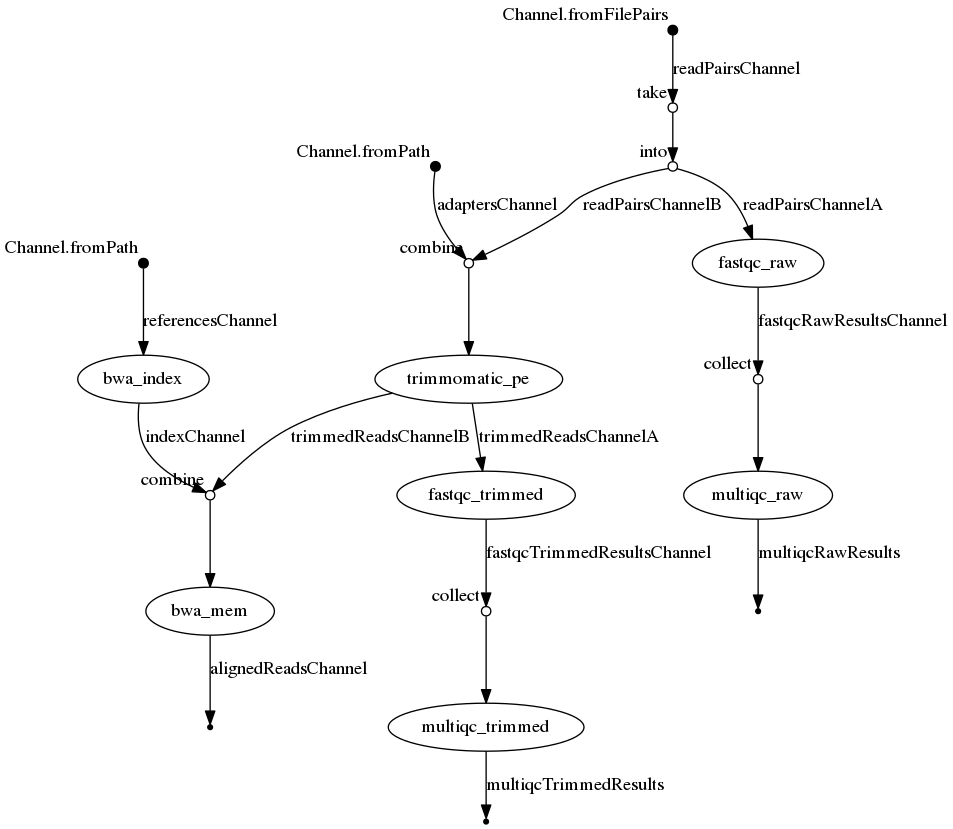
\includegraphics[width=\textwidth]{handout/flowchart.png}
\caption{The example workflow}
\label{fig:dag}
\end{figure}


\begin{questions}
Investigate \texttt{main.nf} alongside Figure~\ref{fig:dag}. 

Which \href{https://www.nextflow.io/docs/latest/operator.html}{nextflow operators}, in addition to the previously discussed, are used and for what purposes? 

\begin{answer}
The \texttt{.combine()} operator outputs all combinations of items emitted by two channels. This results with a downstream process to be executed for each such combination. So e.g. \texttt{bwa\_mem} will be executed for\\ $(reference, accession_1),(reference, accession_2),..,(reference, accession_n)$.

The \texttt{.collect()} operator collects all the items emitted by a channel returns the resulting List as a single emission. This is required e.g. if a process needs to be executed once for all of the samples together.  
\end{answer}

\end{questions}

\subsection{Key concepts to cover}

\begin{itemize}
 \item channels
 \item operators
 \item processes
 \item directives
\end{itemize}

\subsection {Under the hood}



\subsection{Parametrisation}

\begin{itemize}
 \item single dash params
 \item double dash params
 \item environmental variables
\end{itemize}

% To make a paragraph appear as a "note" to the reader, simply wrap it in a "note" environment like
% this:
\begin{note}
Note that currently the default behaviour of Nextflow is to re-run an entire workflow 
unless \texttt{-resume} option is specified at run-time, in which case a previously 
executed process is not re-run if all its remain unchanged.

\end{note}


\subsection{exercises}

\begin{enumerate}
 \item Install NF, run hello example (version run, pull, modify, drop - optional), 
 \item create/modify profile for 
  \item software (conda or singularity)
  \item executor (slurm)
 \item \texttt{publishDir}
 \item process selectors (optional)
\end{enumerate}


%There are 10 characters which have special meaning in \LaTeX and to have them displayed as literal
%characters we need to do something special. The first seven can simply be prepended by a backslash;
%for the other three, we must use the macros \verb+\textasciitilde+, \verb+\textasciicircum+,
%\verb+\textbackslash+.
%
%
%\& \% \$ \# \_ \{ \}
%
%\textasciitilde
%
%\textasciicircum
%
%\textbackslash
%
%Highly redundant coverage ($>$15X) of the genome can be used to correct sequencing
%errors in the reads before assembly and errors. Various k-mer based error
%correction methods exist but are beyond the scope of this tutorial.
%
%In order to use a single character to encode Phred qualities, ASCII characters
%are used (\url{http://shop.alterlinks.com/ascii-table/ascii-table-us.php}). All ASCII characters have a decimal
%number associated with them but the first 32 characters are non-printable (e.g.
%
%Because ASCII characters $<$ 33 are non-printable, using the Phred+33 encoding was
%not possible. Therefore, they simply moved the offset from 33 to 64 thus
%
%schema it is not always possible to identify what encoding is in use. For
%example, if the only characters seen in the quality string are (\texttt{@ABCDEFGHI}),
%then it is impossible to know if you have really good Phred+33 encoded qualities
%or really bad Phred+64 encoded qualities.

%\subsection{Tables}
%
%Writing tables in \LaTeX is HARD! Rather than write them from scratch, I'd head over to
%\url{http://www.tablesgenerator.com/latex_tables}, generate the table you want using the interactive
%page and copy the resulting \LaTeX into your source file.
%
%\begin{tabular}{llr}
%\hline
%\multicolumn{2}{c}{Item} \\
%\cline{1-2}
%Animal    & Description & Price (\$) \\
%\hline
%Gnat      & per gram    & 13.65      \\
%          & each        & 0.01       \\
%Gnu       & stuffed     & 92.50      \\
%Emu       & stuffed     & 33.33      \\
%Armadillo & frozen      & 8.99       \\
%\hline
%\end{tabular}

%\subsection{Figures}
%
%No handout is complete without figures, screenshots or similar.
%
%\begin{figure}[H]
%\centering
%\includegraphics[width=0.8\textwidth]{handout/bad_example.png}
%\caption{Per base sequence quality plot for \texttt{bad\_example.fastq}.}
%\label{fig:bad_example_untrimmed_plot}
%\end{figure}

%\subsection{Maths Environment}
%
%I won't pretend to be an expert in \LaTeX but I do know that one of the strengths of \LaTeX is it's
%ability to allow mathematical formulas to be constructed and typeset very easily. Firstly, you have
%to tell \LaTeX what text is going to contain mathematical symbols.
%
%For inline display, simply surround the relevant text by dollar signs: \verb+$Q(A) =-10 log10(P(\sim A))$+
%
%For more complex mathematical formulas which need to be displayed separately, use the
%\verb+\begin{displaymath} ... \end{displaymath}+ environment to wrap around your formulas.
%
%\begin{displaymath}
%Q(A) =-10 log10(P(\sim A))
%\end{displaymath}





\subsection{Questions and Answers}

It is useful to maintain the answers to questions together in the same \LaTeX source. By using the
\verb+\begin{answer} ... \end{answer}+ environment we can have the enclosed answers excluded from
the trainee's version of the handout while including it in the trainer's version of the handout.

\begin{questions}
We can ask a simply question to test if the trainee is understanding what they are doing.
\begin{answer}
We can maintain the answer along side the questions.
\end{answer}

\end{questions}

%\subsection{Code For Trainees to Copy/Type}
%
%Different people have different opinions on whether it is a good idea to provide the commands for
%trainees to copy-and-paste. In our experience, there is a huge amount of time wasted by novices
%typing commands incorrectly or changing filenames which affects commands you might run later on. We
%also think that it's a good idea to pose regular questions or ask the trainees to modify a previous
%command. This way you can catch out those whoe are just trying to get ahead by blindly
%copying-and-pasting.
%
%To provide a nicely formatted, copy-and-pastable command, simply wrap it in the
%\verb+\begin{lstlisting} ... \end{lstlisting}+ environment. Long commands will be wrapped
%automatically and bash line continuation characters (\textbackslash) inserted where required.
%
%\begin{steps}
%\begin{lstlisting}
%cd ~/QC
%fastx_clipper -h
%fastx_clipper -v -Q 33 -l 20 -M 15 -a GATCGGAAGAGCGGTTCAGCAGGAATGCCGAG -i bad_example.fastq -o bad_example_clipped.fastq
%\end{lstlisting}
%\end{steps}

